\section{Introduction}


Quantile Regression is a powerful tool for measuring quantiles others than the median or predicting the mean. A quantile of a random variable is important in risk measuring, as we can measure the probability of occurrence of extreme events, and in many other fields. While working with energy forecasts, quantile regression can produce interesting results when working with both short term (hourly) or long term (monthly) data. As an example, we present a solar time series for the short term and a wind time series for long term. The first set of data is measured at the location of Tubarao (Brazil) on the year of 2014, while the latter is a dataset of mean power  monthly observations from Icaraizinho (Brazil) between 1981 to 2011 of measured in Megawatts. Figure \ref{fig:boxplots} illustrate the seasonality present in these datasets.

\begin{figure}
	\centering
	\begin{minipage}[t]{\linewidth}
		
		\begin{minipage}[t]{0.45\linewidth}
			%\centering
			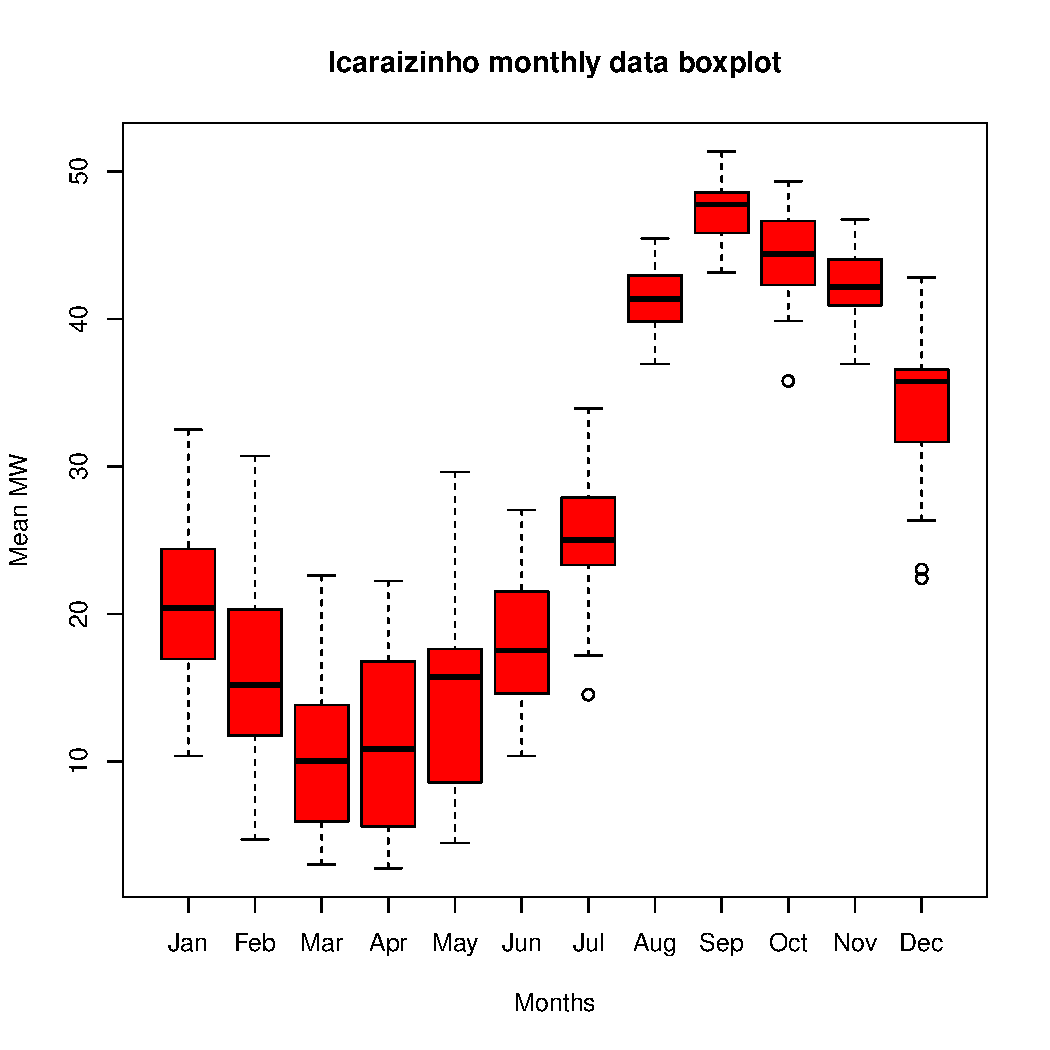
\includegraphics[width=\textwidth]{./../Figuras/Icaraizinho/icaraizinho-boxplot}
			%\caption{Boxplot for each month for the Icaraizinho dataset}
			\label{fig:icaraizinho-boxplot}
		\end{minipage}
		\begin{minipage}[t]{0.45\linewidth}
			%\centering
			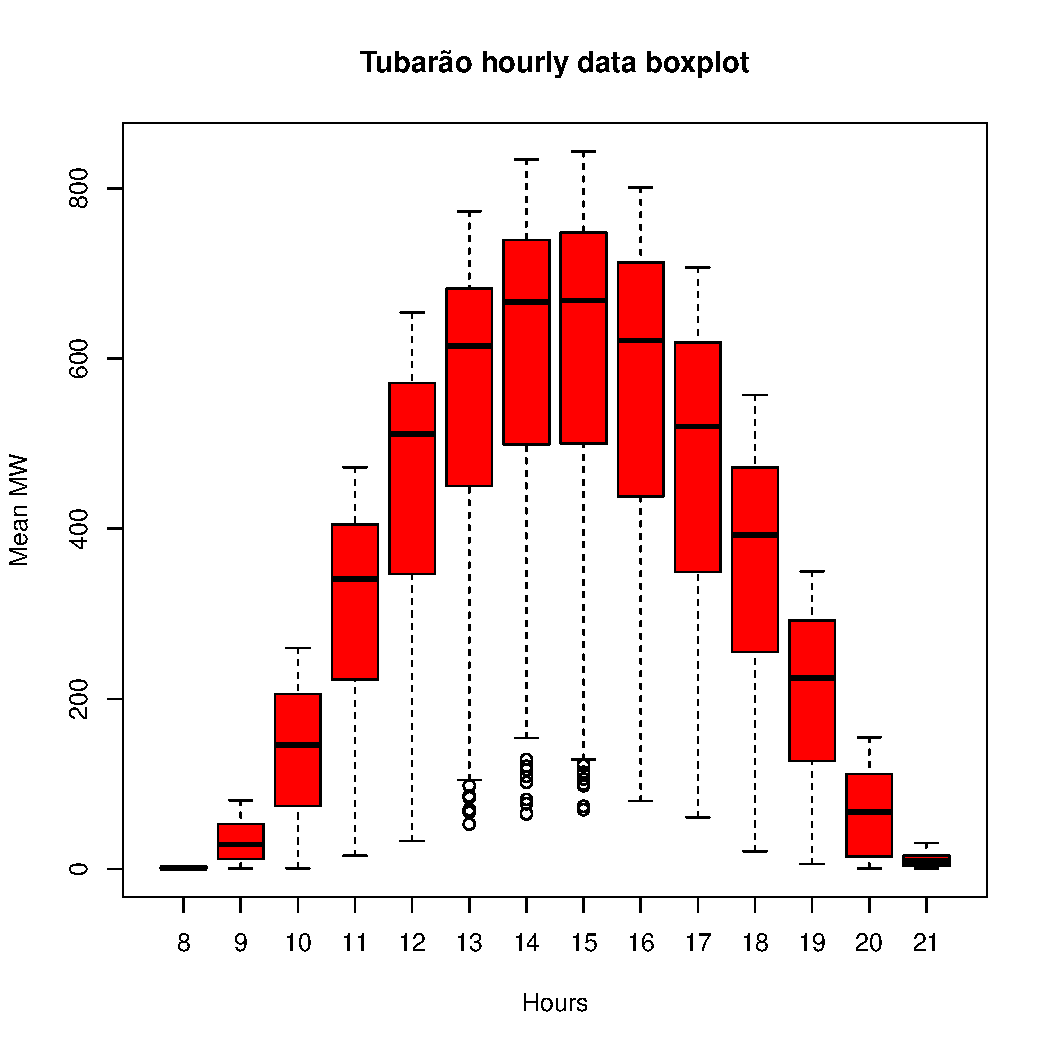
\includegraphics[width=\textwidth]{./../Figuras/Solar-exemplos/tubarao-boxplot}
			%\caption{Boxplot for each month for the Icaraizinho dataset}
			\label{fig:tubarao-boxplot}
		\end{minipage}
	\end{minipage}
	\caption{Boxplots showing seasonality for monthly and hourly data.}
	\label{fig:boxplots}
\end{figure}

Let $Y$ be a real valued random variable. The quantile function $Q_Y:[0,1] \rightarrow \mathbb{R}$ is defined pointwise by its $\alpha$-quantile, which is given by
\begin{equation}
Q_Y(\alpha) = F_Y^{-1}(\alpha) = \inf\{y: F_Y(y) \geq \alpha\},
\label{eq:quantile-function}
\end{equation}
where $F_Y$ is the distribution function of random variable $Y$ and $\alpha \in [0,1]$. Equation \ref{eq:quantile-function} defines what we call from now on as the quantile function $Q_Y(\cdot)$, in relation to random variable $Y$. In this article, we are interested in a conditional quantile function $Q_{Y|X=x}:[0,1] \times \mathbb{R}^d \rightarrow \mathbb{R}$ (in short, from now on, $Q_{Y|X}(\cdot, \cdot)$), where $X$ can be a vector.

Let $(\Omega, \mathcal{F}, P)$ be a probability space. The conditional quantile function can be found as the result of the following optimization problem:
\begin{eqnarray}
Q_{Y|X}(\alpha, \cdot)\quad & \in\quad\underset{q_\alpha(\cdot)}{\text{arg min}}\, &
(1-\alpha)\int_{\omega \in \Omega}|Y(w)-q_\alpha(X(w))|^{-}P(dw) \label{eq:optim-continuous}
\\ & & + (\alpha)\int_{\omega \in \Omega}|Y(w)-q_\alpha(X(w))|^{+}P(dw) \nonumber
\end{eqnarray}

\begin{equation}
q_\alpha  \in \mathcal{Q},
\end{equation}
The argument of optimization problem described on equation \ref{eq:optim-continuous} is the function $q_\alpha$, which belongs to a function space $\mathcal{Q}$. We might have different assumptions for the space $\mathcal{Q}$, depending on the type of function we want to find for $q_\alpha$. A few properties, however, must be achieved by our choice. The conditional quantile function $Q_{Y|X}(\alpha)$ must be monotone on $\alpha$, and its first derivative must be limited.


In this work, we use the sample quantile,  where we calculate the optimization based on a finite number of observations, instead of integrating over all domain of random variable $Y$. For the specific case where the random variable is a time series $y_t$, quantiles are estimated from a $n$ size sample of observations of $y_t$ and a explanatory variable $x_t$ for each $t$, such that our random sample is formed by the sequence $\{y_t,x_t \}_{t=1}^n$. To estimate the $\alpha$-quantile from a sample, we change \ref{eq:optim-continuous} for the following optimization problem:
\begin{equation}
\hat{Q}_{Y|X}(\alpha, \cdot)\quad \in\quad\underset{q_\alpha(\cdot)}{\text{arg min}}\,\sum_{t \in T}\alpha|y_{t}-q_\alpha(\cdot)|^{+}+\sum_{t \in T}(1-\alpha)|y_{t}-q_\alpha(\cdot)|^{-},
\label{eq:linear-model}
\end{equation}
\begin{equation}
q_\alpha  \in \mathcal{Q},
\end{equation}
where $T = \{1, \dots, n \}$, $|x|^+=\max\{0,x\}$ and $|x|^-=-\min\{0,x\}$. The solution from the above problem is an estimator $\hat{Q}_{Y|X}$ for the quantile function $Q_{Y|X}$.

To model this problem as a Linear Programming problem, thus being able to use a modern solver to fit our model,  we create variables $\varepsilon^+_t$ e $\varepsilon^-_t$ to represent $|y-q(\cdot)|^+$ and $|y-q(\cdot)|^-$, respectively. The optimal argument $q_\alpha^*(\cdot)$ on the Linear Programming problem \ref{eq:qar-general} is the estimated $\alpha$-quantile for the given random sample.
\begin{equation}
\begin{aligned}q^*_\alpha(.) \in \underset{q_\alpha (\cdot),\varepsilon_{t}^{+}, \varepsilon_{t}^{-}}{\text{arg min}} & \sum_{t \in T}\left(\alpha \varepsilon_{t}^{+}+(1-\alpha)\varepsilon_{t}^{-}\right) & \\
\mbox{s.t. } & \varepsilon_{t}^{+}-\varepsilon_{t}^{-}=y_{t}-q_\alpha(x_t), & \qquad\forall t \in T,\\
& \varepsilon_t^+,\varepsilon_t^- \geq 0, & \qquad \forall t \in T.
\end{aligned}
\label{eq:qar-general}
\end{equation}

Let $A$ be a set containing a sequence of probabilities  $\alpha_i$ such that $0 < \alpha_1 < \alpha_2 < \dots < \alpha_Q < 1$. This set represents a finite discretization of the interval $[0,1]$.
One of our goals with quantile regression is to estimate a quantile function $\hat{Q}_{Y|X}$ of a given real valued random variable $X$ from a sequence of quantiles $q_{\alpha_1}(x_t) \leq q_{\alpha_2}(x_t) \leq \dots \leq q_{\alpha_{|A|}}(x_t)$, with $0 < \alpha_1 < \alpha_2 < \dots < \alpha_{|A|} < 1$, for any given $t$.
The process of fitting $\hat{Q}_{Y|X}$ is by mapping every $\alpha_i$ with its estimated quantile $\hat{q}_{\alpha_i}(x_t)$.
The denser the grid of values in $A$, better is the approximation of $Q_{Y|X}$.
Thus, the distribution found for $Y$ is nonparametric, as no previous assumptions are made about its shape, and its form is fully recovered by the data we have.

A typical problem, however, arises when working with quantile regression. When quantiles are estimated independently, it is possible to find $q_{\alpha}(x_t) > q_{\alpha'}(x_t)$, for a given $t$, when $\alpha_1 < \alpha_2$. An example can be seen on Figure \ref{fig:crossing-quantiles}, where quantiles $\alpha = 0.95$ and $\alpha = 0.9$ cross. This problem, called \textit{crossing quantiles}, can be prevented by estimating all quantiles with a single minimization problem.
\begin{figure}
	\centering
	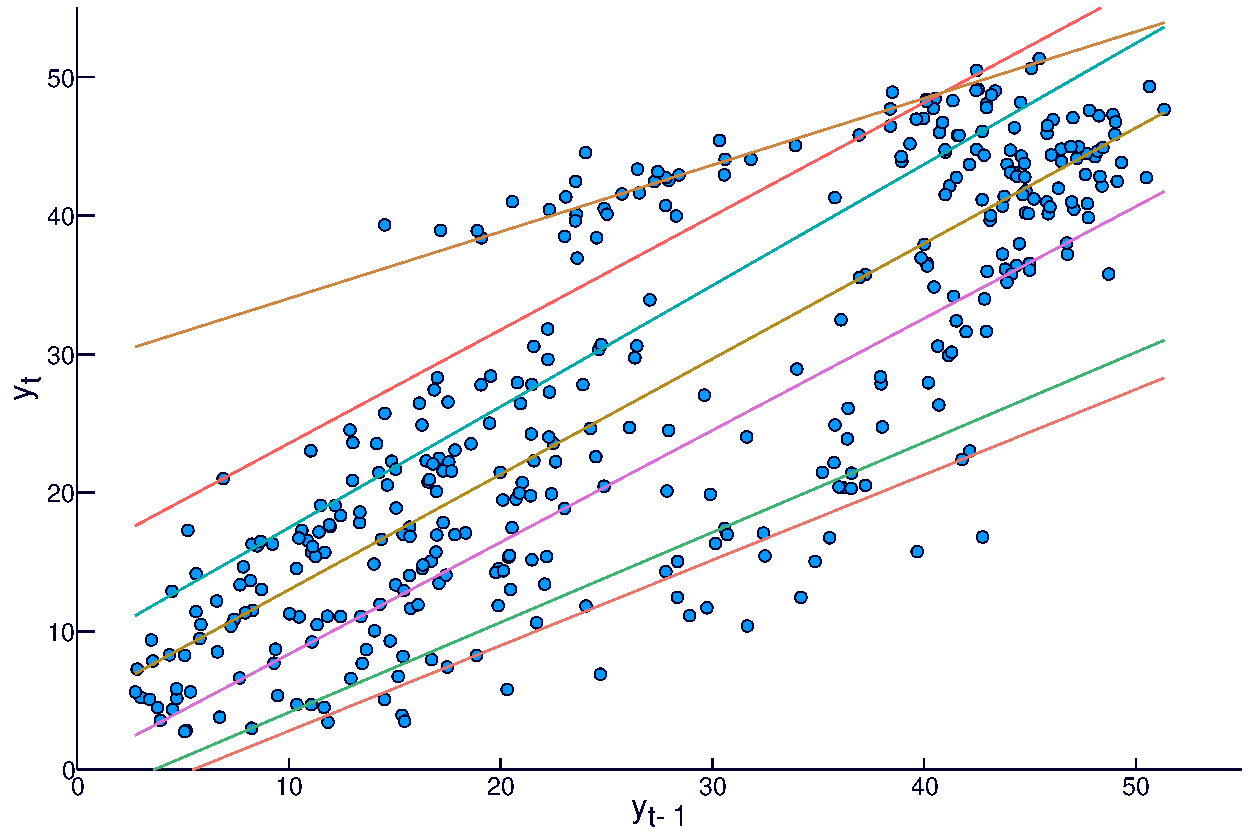
\includegraphics[width=0.6\linewidth]{./../Figuras/regressao-quantilica/icaraizinho-quantile-linear-scatter-crossing}
	\caption{Linear quantile estimator with crossing quantiles for $\alpha = 0.95$ and $\alpha = 0.9$}
	\label{fig:crossing-quantiles}
\end{figure}

In order to estimate all quantiles simultaneously, the new objective function will be the sum of all individual objective functions, as well as include all constraints from all individual problems. The only difference is the inclusion of an equation to guarantee that quantiles won't cross.  When modifying problem \ref{eq:qar-general} to account for all quantiles, we have the following new problem:
\begin{eqnarray}
\label{eq:non-crossing-quantiles1}
\{q^*_{\alpha}(\cdot)\}_{\alpha \in A}  \in \underset{q_\alpha(\cdot),\varepsilon_{t \alpha}^{+}, \varepsilon_{t \alpha}^-}{\text{arg min}} &  \sum_{\alpha \in A} \sum_{t \in T}\left(\alpha \varepsilon_{t \alpha}^++(1-\alpha)\varepsilon_{t \alpha}^{-}\right) &  \\
\mbox{s.t. } & \varepsilon_{t \alpha}^{+}-\varepsilon_{t \alpha}^{-}=y_{t}-q_\alpha(x_{t}), & \qquad\forall t \in T,\forall \alpha \in A,\\
& \varepsilon_{t \alpha}^+,\varepsilon_{t \alpha}^- \geq 0, & \qquad\forall t \in T,\forall \alpha \in A,\\\label{eq:non-crossing-constraint}
& q_{\alpha}(x_t) \leq q_{\alpha'}(x_t), & \qquad \forall t \in T, \forall (\alpha, \alpha') \in A \times A,  \alpha' > \alpha,\nonumber\\
\end{eqnarray}
where constraint \ref{eq:non-crossing-constraint} assures that no lower quantile will have a bigger value than a higher quantile.




The next section discusses with bigger details how to fit a distribution function $Q_{Y|X}(\alpha,x)$ from a sequence of estimated quantiles, as well as showing two different strategies to estimate them: linear models and nonparametric models. In the former, $q_\alpha$ is a linear function of an explanatory variable $x_t$.
In the latter, we let $q_\alpha(x_t)$ assume any functional form. To prevent overfitting, however, we penalize the function's roughness by incorporating a penalty on the second derivative.


% % % % % % % % % % % % % % % % % % %

As opposed to the conventional work of doing a model to forecast the
conditional mean, our work focus on finding a distribution for $y_{t}$
on each $t$. 

We find a time series model, based on quantile autoregression (as
in Konker 2005).

As we are interested in the whole distribution of $\hat{y}_{t+k|t}$,
we estimate a phin grid of quantiles in $0<\alpha_{1}<\alpha_{2}<\dots<\alpha_{|A|}<1$,
such that the distribution can be well approximated.

As a Quantile Autoregression model, we are interested in selecting
the best subset of variables do model the time series. 

As we are trying to model the whole $k$-step ahead distribution,
we estimate many quantiles. We didn't find any previous work where
a given $\alpha$-quantile model influenced another model.

In all works found, each quantile is estimated separately. 

Regularization can be done by introducing a penalty on the $\ell_1$-norm of the coefficients. The work by \cite{belloni_l1-penalized_2009} defines proprieties and convergence analysis. The AdaLasso variant, where each coefficient may have a different weight on the objective function to ensure oracle proprieties, is developed on \cite{ciuperca_adaptive_2016}.